\documentclass[../main.tex]{subfiles}

\begin{document}

\subsection{Modelando con Markov}

\paragraph{} Problemas como el anterior se pueden representar con lo que se conoce como un modelo de Markov. Donde tenemos un estado que cambia aleatoriamente en base al estado anterior.

El caso anterior es complicado de representar, por lo que vamos a ver a otro sistema más fácil de representar.

\paragraph{} Vamos a modelar a un robot que se mueve sobre un tablero como el del ajedrez.  En específico va a empezar en la posición \(\GTuple{0}{0}\) en un tablero de \(3 \times 3\). En cada paso elije al azar a dónde se mueve entre los casilleros que tenga al lado. Se busca saber la probabilidad de que esté en algún casillero específico después de \(k\) pasos.

\paragraph{} Primero probemos simularlo a mano dibujando sus posibles caminos para un par de pasos:

Inicialmente sabemos que se encuentra en \(\GTuple{0}{0}\).

\begin{figure}[H]
  \centering
  \begin{tikzpicture}
    \CVertex{a1}{0}{0}{0}
  \end{tikzpicture}
  \caption{Posición inicial del robot.}
\end{figure}

Luego del primer paso tiene probabilidad \(\frac{1}{2}\) de encontrarse en \(\GTuple{0}{1}\) y \(\frac{1}{2}\) de encontrarse en \(\GTuple{1}{0}\).

\begin{figure}[H]
  \centering
  \begin{tikzpicture}
    \CVertex{a1}{0}{0}{0}
      \CVertex{a2}{-3}{-3}{1}
      \CVertex{b1}{3}{-3}{2}

    \GEdge{$\frac{1}{2}$}{0}{1}
    \GEdge{$\frac{1}{2}$}{0}{2}
  \end{tikzpicture}
  \caption{Paso uno.}
\end{figure}

Y luego del segundo paso tiene probabilidad \(\frac{1}{3}\) de encontrarse en \(\GTuple{0}{0}\), \(\frac{1}{3}\) de encontrarse en \(\GTuple{1}{1}\), \(\frac{1}{6}\) de encontrarse en \(\frac{2}{0}\), y \(\frac{1}{6}\) de encontrarse en \(\GTuple{0}{2}\).

\begin{figure}[H]
  \centering
  \begin{tikzpicture}
    \CVertex{a1}{0}{0}{0}
      \CVertex{a2}{-3}{-3}{1}
        \CVertex{a3}{-6}{-6}{3}
        \CVertex{b2}{0}{-6}{4}
      \CVertex{b1}{3}{-3}{2}
        \CVertex{c1}{6}{-6}{5}

    \GEdge{$\frac{1}{2} \cdot \frac{1}{3}$}{1}{0}
    \GEdge{$\frac{1}{2} \cdot \frac{1}{3}$}{1}{3}
    \GEdge{$\frac{1}{2} \cdot \frac{1}{3}$}{1}{4}

    \GEdge{$\frac{1}{2} \cdot \frac{1}{3}$}{2}{0}
    \GEdge{$\frac{1}{2} \cdot \frac{1}{3}$}{2}{4}
    \GEdge{$\frac{1}{2} \cdot \frac{1}{3}$}{2}{5}
  \end{tikzpicture}
  \caption{Paso dos.}
\end{figure}

\paragraph{} Ahora entonces defino al vector \(v_{k}\) tal que \((v_{k})_{i} = P(\text{El robot esté en la posición } i \text{ después del paso } k)\), o sea que representa la distribución de la posición del robot después del \(k\)-ésimo paso.

Enumerando a las posiciones de la forma \(\GTuple{r}{c} = 3r + c\).

Por lo que los vectores \(v_{0}\), \(v_{1}\), y \(v_{2}\) quedarían así:

\begin{align*}
  v_{0} &= \begin{pmatrix}
    1 \\
    0 \\
    0 \\
    0 \\
    0 \\
    0 \\
    0 \\
    0 \\
    0
  \end{pmatrix} &
  v_{1} &= \begin{pmatrix}
    0 \\
    \frac{1}{2} \\
    0 \\
    \frac{1}{2} \\
    0 \\
    0 \\
    0 \\
    0 \\
    0
  \end{pmatrix} &
  v_{2} &= \begin{pmatrix}
    \frac{1}{3} \\
    0 \\
    \frac{1}{6} \\
    0 \\
    \frac{1}{3} \\
    0 \\
    \frac{1}{6} \\
    0 \\
    0
  \end{pmatrix}
\end{align*}

\paragraph{} Ahora podemos entonces ver estos vectores y los movimientos del robot de una forma más práctica:

\begin{figure}[H]
  \centering
  \begin{tikzpicture}
    \GVertex{1}{0}{0}{0}
    \GVertex{0}{2}{0}{1}
    \GVertex{0}{4}{0}{2}

    \GVertex{0}{0}{2}{3}
    \GVertex{0}{2}{2}{4}
    \GVertex{0}{4}{2}{5}

    \GVertex{0}{0}{4}{6}
    \GVertex{0}{2}{4}{7}
    \GVertex{0}{4}{4}{8}
  \end{tikzpicture}
  \caption{Paso cero.}
\end{figure}

\begin{figure}[H]
  \centering
  \begin{tikzpicture}
    \GVertex{0}{0}{0}{0}
    \GVertex{$\frac{1}{2}$}{2}{0}{1}
    \GVertex{0}{4}{0}{2}

    \GVertex{$\frac{1}{2}$}{0}{2}{3}
    \GVertex{0}{2}{2}{4}
    \GVertex{0}{4}{2}{5}

    \GVertex{0}{0}{4}{6}
    \GVertex{0}{2}{4}{7}
    \GVertex{0}{4}{4}{8}

    \GEdge{$\frac{1}{2}$}{0}{1}
    \GEdge{$\frac{1}{2}$}{0}{3}
  \end{tikzpicture}
  \caption{Paso uno.}
\end{figure}

\begin{figure}[H]
  \centering
  \begin{tikzpicture}
    \GVertex{$\frac{1}{3}$}{0}{0}{0}
    \GVertex{0}{2}{0}{1}
    \GVertex{$\frac{1}{6}$}{4}{0}{2}

    \GVertex{0}{0}{2}{3}
    \GVertex{$\frac{1}{3}$}{2}{2}{4}
    \GVertex{0}{4}{2}{5}

    \GVertex{$\frac{1}{6}$}{0}{4}{6}
    \GVertex{0}{2}{4}{7}
    \GVertex{0}{4}{4}{8}

    \GEdge{$\frac{1}{3}$}{1}{0}
    \GEdge{$\frac{1}{3}$}{1}{2}
    \GEdge{$\frac{1}{3}$}{1}{4}

    \GEdge{$\frac{1}{3}$}{3}{0}
    \GEdge{$\frac{1}{3}$}{3}{4}
    \GEdge{$\frac{1}{3}$}{3}{6}
  \end{tikzpicture}
  \caption{Paso dos.}
\end{figure}

\paragraph{} Y de forma general podemos ver para cada posición los movimientos posibles:

\begin{figure}[H]
  \centering
  \begin{tikzpicture}
    \GVertex{\phantom{0}}{0}{0}{0}
    \GVertex{\phantom{0}}{2}{0}{1}
    \GVertex{\phantom{0}}{4}{0}{2}

    \GVertex{\phantom{0}}{0}{2}{3}
    \GVertex{\phantom{0}}{2}{2}{4}
    \GVertex{\phantom{0}}{4}{2}{5}

    \GVertex{\phantom{0}}{0}{4}{6}
    \GVertex{\phantom{0}}{2}{4}{7}
    \GVertex{\phantom{0}}{4}{4}{8}

    \GBEdge{$\frac{1}{2}$}{0}{1}
    \GBEdge{$\frac{1}{2}$}{0}{3}

    \GBEdge{$\frac{1}{3}$}{1}{0}
    \GBEdge{$\frac{1}{3}$}{1}{2}
    \GBEdge{$\frac{1}{3}$}{1}{4}

    \GBEdge{$\frac{1}{2}$}{2}{1}
    \GBEdge{$\frac{1}{2}$}{2}{5}

    \GBEdge{$\frac{1}{3}$}{3}{0}
    \GBEdge{$\frac{1}{3}$}{3}{4}
    \GBEdge{$\frac{1}{3}$}{3}{6}

    \GBEdge{$\frac{1}{4}$}{4}{1}
    \GBEdge{$\frac{1}{4}$}{4}{3}
    \GBEdge{$\frac{1}{4}$}{4}{5}
    \GBEdge{$\frac{1}{4}$}{4}{7}

    \GBEdge{$\frac{1}{3}$}{5}{2}
    \GBEdge{$\frac{1}{3}$}{5}{4}
    \GBEdge{$\frac{1}{3}$}{5}{8}

    \GBEdge{$\frac{1}{2}$}{6}{3}
    \GBEdge{$\frac{1}{2}$}{6}{7}

    \GBEdge{$\frac{1}{3}$}{7}{4}
    \GBEdge{$\frac{1}{3}$}{7}{6}
    \GBEdge{$\frac{1}{3}$}{7}{8}

    \GBEdge{$\frac{1}{2}$}{8}{5}
    \GBEdge{$\frac{1}{2}$}{8}{7}
  \end{tikzpicture}
\end{figure}

\paragraph{} Y siendo que representamos al estado después del \(k\)-ésimo paso como un vector, podemos armar una matriz de transición que aplique los movimientos posibles sobre el vector.

\begin{gather*}
  \overbrace{\begin{pmatrix}
      0 & \frac{1}{3} & 0 & \frac{1}{3} & 0 & 0 & 0 & 0 & 0  \\
      \frac{1}{2} & 0 & \frac{1}{2} & 0 & \frac{1}{4} & 0 & 0 & 0 & 0  \\
      0 & \frac{1}{3} & 0 & 0 & 0 & \frac{1}{3} & 0 & 0 & 0  \\
      \frac{1}{2} & 0 & 0 & 0 & \frac{1}{4} & 0 & \frac{1}{2} & 0 & 0  \\
      0 & \frac{1}{3} & 0 & \frac{1}{3} & 0 & \frac{1}{3} & 0 & \frac{1}{3} & 0  \\
      0 & 0 & \frac{1}{2} & 0 & \frac{1}{4} & 0 & 0 & 0 & \frac{1}{2} \\
      0 & 0 & 0 & \frac{1}{3} & 0 & 0 & 0 & \frac{1}{3} & 0  \\
      0 & 0 & 0 & 0 & \frac{1}{4} & 0 & \frac{1}{2} & 0 & \frac{1}{2} \\
      0 & 0 & 0 & 0 & 0 & \frac{1}{3} & 0 & \frac{1}{3} & 0
  \end{pmatrix}}^{\text{Matriz de transición}}
  \overbrace{\begin{pmatrix}
      1 \\ 0 \\ 0 \\ 0 \\ 0 \\ 0 \\ 0 \\ 0 \\ 0 
  \end{pmatrix}}^{\text{Este estado (\(\langle 0, 0 \rangle\))}}
  =
  \overbrace{\begin{pmatrix}
      0 \\ \frac{1}{2} \\ 0 \\ \frac{1}{2} \\ 0 \\ 0 \\ 0 \\ 0 \\ 0 
  \end{pmatrix}}^{\text{Siguiente estado}}
\end{gather*}

\paragraph{} Y en general, como la matriz de transición no cambia entre pasos, se vale que:

\begin{gather*}
  M^{k} v_{0} = \overbrace{v_{k}}^{\text{Distribución del \(k\)-ésimo estado}}
\end{gather*} 

Por lo que el resultado a lo pedido es
\begin{gather*}
  P(\text{Esté en la posición } \langle r, c \rangle \text{ en el \(k\)-ésimo paso}) = (M^{k}v_{0})_{3r + c} = (v_{k})_{3r + c}
\end{gather*}

\end{document}
